% Created by tikzDevice version 0.12.6 on 2024-10-23 10:54:38
% !TEX encoding = UTF-8 Unicode
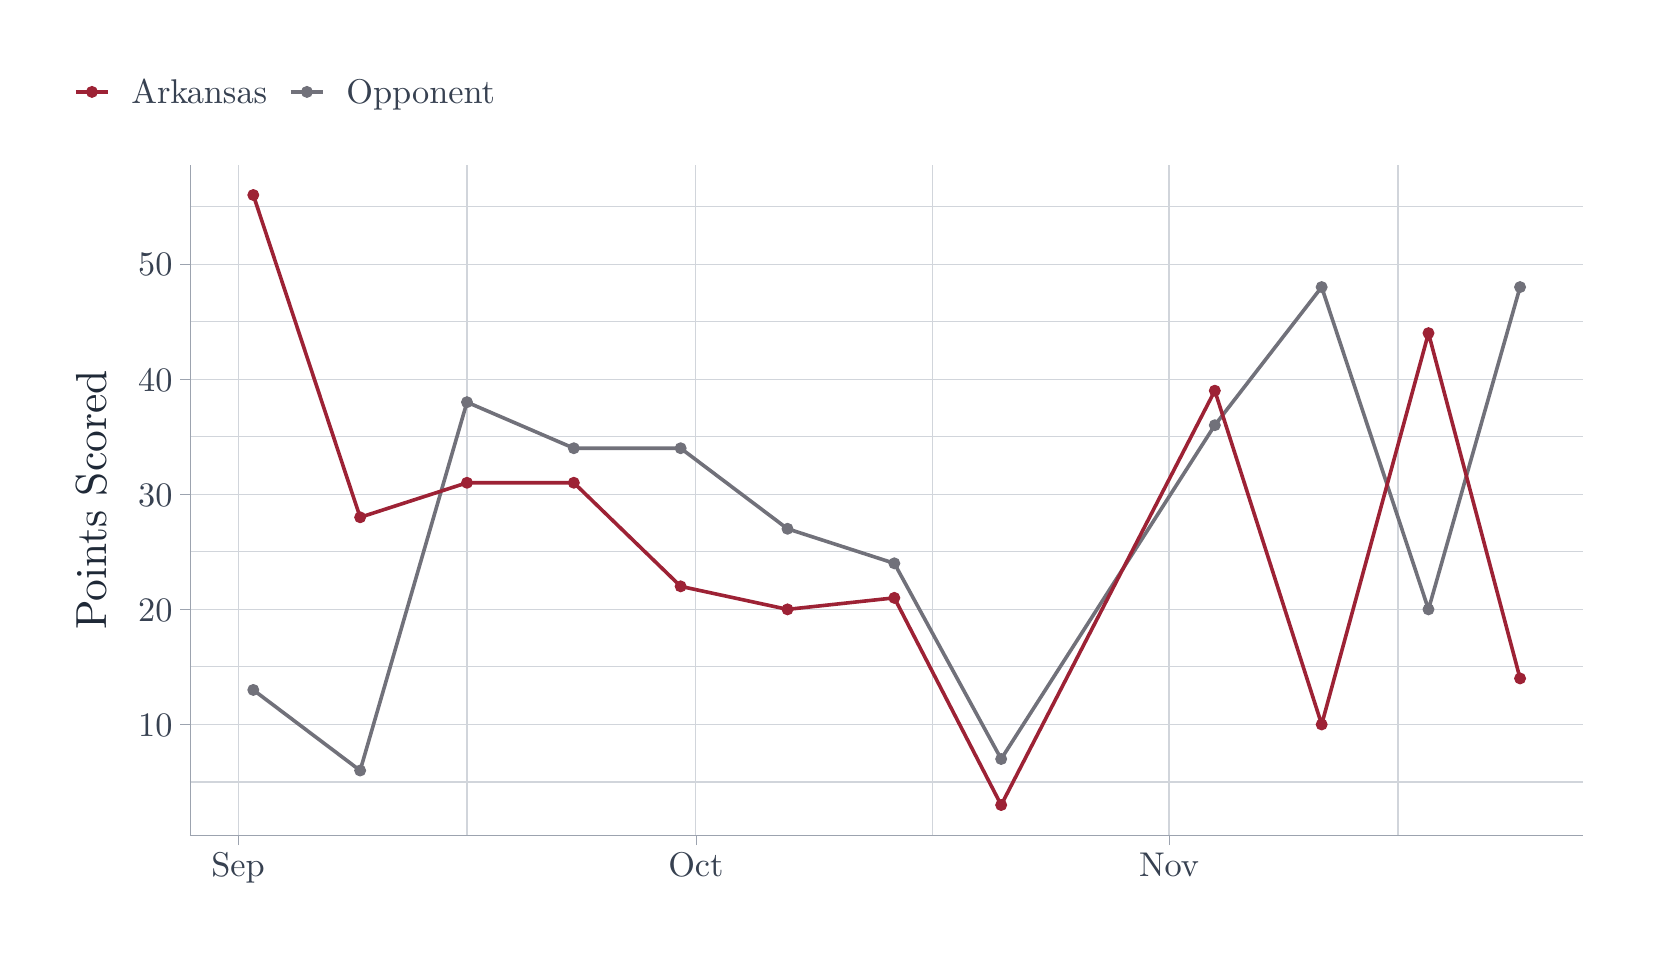
\begin{tikzpicture}[x=1pt,y=1pt]
\definecolor{fillColor}{RGB}{255,255,255}
\path[use as bounding box,fill=fillColor] (0,0) rectangle (578.16,325.21);
\begin{scope}
\path[clip] (  0.00,  0.00) rectangle (578.16,325.21);
\definecolor{drawColor}{RGB}{255,255,255}

\path[draw=drawColor,line width= 0.7pt,line join=round,line cap=round,fill=fillColor] (  0.00,  0.00) rectangle (578.16,325.21);
\end{scope}
\begin{scope}
\path[clip] ( 58.65, 33.29) rectangle (562.16,275.76);
\definecolor{drawColor}{RGB}{255,255,255}
\definecolor{fillColor}{RGB}{255,255,255}

\path[draw=drawColor,line width= 0.7pt,line join=round,line cap=round,fill=fillColor] ( 58.65, 33.29) rectangle (562.16,275.76);
\definecolor{drawColor}{RGB}{209,213,219}

\path[draw=drawColor,line width= 0.4pt,line join=round] ( 58.65, 52.63) --
	(562.16, 52.63);

\path[draw=drawColor,line width= 0.4pt,line join=round] ( 58.65, 94.22) --
	(562.16, 94.22);

\path[draw=drawColor,line width= 0.4pt,line join=round] ( 58.65,135.81) --
	(562.16,135.81);

\path[draw=drawColor,line width= 0.4pt,line join=round] ( 58.65,177.40) --
	(562.16,177.40);

\path[draw=drawColor,line width= 0.4pt,line join=round] ( 58.65,218.99) --
	(562.16,218.99);

\path[draw=drawColor,line width= 0.4pt,line join=round] ( 58.65,260.58) --
	(562.16,260.58);

\path[draw=drawColor,line width= 0.4pt,line join=round] (158.74, 33.29) --
	(158.74,275.76);

\path[draw=drawColor,line width= 0.4pt,line join=round] (326.95, 33.29) --
	(326.95,275.76);

\path[draw=drawColor,line width= 0.4pt,line join=round] (495.15, 33.29) --
	(495.15,275.76);

\path[draw=drawColor,line width= 0.4pt,line join=round] ( 58.65, 73.42) --
	(562.16, 73.42);

\path[draw=drawColor,line width= 0.4pt,line join=round] ( 58.65,115.01) --
	(562.16,115.01);

\path[draw=drawColor,line width= 0.4pt,line join=round] ( 58.65,156.60) --
	(562.16,156.60);

\path[draw=drawColor,line width= 0.4pt,line join=round] ( 58.65,198.19) --
	(562.16,198.19);

\path[draw=drawColor,line width= 0.4pt,line join=round] ( 58.65,239.78) --
	(562.16,239.78);

\path[draw=drawColor,line width= 0.4pt,line join=round] ( 76.02, 33.29) --
	( 76.02,275.76);

\path[draw=drawColor,line width= 0.4pt,line join=round] (241.47, 33.29) --
	(241.47,275.76);

\path[draw=drawColor,line width= 0.4pt,line join=round] (412.43, 33.29) --
	(412.43,275.76);
\definecolor{drawColor}{RGB}{113,113,122}

\path[draw=drawColor,line width= 1.3pt,line join=round] ( 81.53, 85.90) --
	(120.14, 56.78) --
	(158.74,189.88) --
	(197.35,173.24) --
	(235.95,173.24) --
	(274.56,144.13) --
	(313.16,131.65) --
	(351.77, 60.94) --
	(428.97,181.56) --
	(467.58,231.47) --
	(506.18,115.01) --
	(539.27,231.47);
\definecolor{fillColor}{RGB}{113,113,122}

\path[draw=drawColor,line width= 0.4pt,line join=round,line cap=round,fill=fillColor] (467.58,231.47) circle (  1.96);

\path[draw=drawColor,line width= 0.4pt,line join=round,line cap=round,fill=fillColor] (428.97,181.56) circle (  1.96);

\path[draw=drawColor,line width= 0.4pt,line join=round,line cap=round,fill=fillColor] (197.35,173.24) circle (  1.96);

\path[draw=drawColor,line width= 0.4pt,line join=round,line cap=round,fill=fillColor] ( 81.53, 85.90) circle (  1.96);

\path[draw=drawColor,line width= 0.4pt,line join=round,line cap=round,fill=fillColor] (274.56,144.13) circle (  1.96);

\path[draw=drawColor,line width= 0.4pt,line join=round,line cap=round,fill=fillColor] (158.74,189.88) circle (  1.96);

\path[draw=drawColor,line width= 0.4pt,line join=round,line cap=round,fill=fillColor] (120.14, 56.78) circle (  1.96);

\path[draw=drawColor,line width= 0.4pt,line join=round,line cap=round,fill=fillColor] (351.77, 60.94) circle (  1.96);

\path[draw=drawColor,line width= 0.4pt,line join=round,line cap=round,fill=fillColor] (539.27,231.47) circle (  1.96);

\path[draw=drawColor,line width= 0.4pt,line join=round,line cap=round,fill=fillColor] (313.16,131.65) circle (  1.96);

\path[draw=drawColor,line width= 0.4pt,line join=round,line cap=round,fill=fillColor] (506.18,115.01) circle (  1.96);

\path[draw=drawColor,line width= 0.4pt,line join=round,line cap=round,fill=fillColor] (235.95,173.24) circle (  1.96);
\definecolor{drawColor}{RGB}{157,34,53}

\path[draw=drawColor,line width= 1.3pt,line join=round] ( 81.53,264.74) --
	(120.14,148.28) --
	(158.74,160.76) --
	(197.35,160.76) --
	(235.95,123.33) --
	(274.56,115.01) --
	(313.16,119.17) --
	(351.77, 44.31) --
	(428.97,194.03) --
	(467.58, 73.42) --
	(506.18,214.83) --
	(539.27, 90.06);
\definecolor{fillColor}{RGB}{157,34,53}

\path[draw=drawColor,line width= 0.4pt,line join=round,line cap=round,fill=fillColor] (467.58, 73.42) circle (  1.96);

\path[draw=drawColor,line width= 0.4pt,line join=round,line cap=round,fill=fillColor] (428.97,194.03) circle (  1.96);

\path[draw=drawColor,line width= 0.4pt,line join=round,line cap=round,fill=fillColor] (197.35,160.76) circle (  1.96);

\path[draw=drawColor,line width= 0.4pt,line join=round,line cap=round,fill=fillColor] ( 81.53,264.74) circle (  1.96);

\path[draw=drawColor,line width= 0.4pt,line join=round,line cap=round,fill=fillColor] (274.56,115.01) circle (  1.96);

\path[draw=drawColor,line width= 0.4pt,line join=round,line cap=round,fill=fillColor] (158.74,160.76) circle (  1.96);

\path[draw=drawColor,line width= 0.4pt,line join=round,line cap=round,fill=fillColor] (120.14,148.28) circle (  1.96);

\path[draw=drawColor,line width= 0.4pt,line join=round,line cap=round,fill=fillColor] (351.77, 44.31) circle (  1.96);

\path[draw=drawColor,line width= 0.4pt,line join=round,line cap=round,fill=fillColor] (539.27, 90.06) circle (  1.96);

\path[draw=drawColor,line width= 0.4pt,line join=round,line cap=round,fill=fillColor] (313.16,119.17) circle (  1.96);

\path[draw=drawColor,line width= 0.4pt,line join=round,line cap=round,fill=fillColor] (506.18,214.83) circle (  1.96);

\path[draw=drawColor,line width= 0.4pt,line join=round,line cap=round,fill=fillColor] (235.95,123.33) circle (  1.96);
\end{scope}
\begin{scope}
\path[clip] (  0.00,  0.00) rectangle (578.16,325.21);
\definecolor{drawColor}{RGB}{156,163,175}

\path[draw=drawColor,line width= 0.3pt,line join=round] ( 58.65, 33.29) --
	( 58.65,275.76);
\end{scope}
\begin{scope}
\path[clip] (  0.00,  0.00) rectangle (578.16,325.21);
\definecolor{drawColor}{RGB}{55,65,81}

\node[text=drawColor,anchor=base east,inner sep=0pt, outer sep=0pt, scale=  1.24] at ( 52.35, 69.14) {10};

\node[text=drawColor,anchor=base east,inner sep=0pt, outer sep=0pt, scale=  1.24] at ( 52.35,110.73) {20};

\node[text=drawColor,anchor=base east,inner sep=0pt, outer sep=0pt, scale=  1.24] at ( 52.35,152.32) {30};

\node[text=drawColor,anchor=base east,inner sep=0pt, outer sep=0pt, scale=  1.24] at ( 52.35,193.91) {40};

\node[text=drawColor,anchor=base east,inner sep=0pt, outer sep=0pt, scale=  1.24] at ( 52.35,235.50) {50};
\end{scope}
\begin{scope}
\path[clip] (  0.00,  0.00) rectangle (578.16,325.21);
\definecolor{drawColor}{RGB}{156,163,175}

\path[draw=drawColor,line width= 0.3pt,line join=round] ( 55.15, 73.42) --
	( 58.65, 73.42);

\path[draw=drawColor,line width= 0.3pt,line join=round] ( 55.15,115.01) --
	( 58.65,115.01);

\path[draw=drawColor,line width= 0.3pt,line join=round] ( 55.15,156.60) --
	( 58.65,156.60);

\path[draw=drawColor,line width= 0.3pt,line join=round] ( 55.15,198.19) --
	( 58.65,198.19);

\path[draw=drawColor,line width= 0.3pt,line join=round] ( 55.15,239.78) --
	( 58.65,239.78);
\end{scope}
\begin{scope}
\path[clip] (  0.00,  0.00) rectangle (578.16,325.21);
\definecolor{drawColor}{RGB}{156,163,175}

\path[draw=drawColor,line width= 0.3pt,line join=round] ( 58.65, 33.29) --
	(562.16, 33.29);
\end{scope}
\begin{scope}
\path[clip] (  0.00,  0.00) rectangle (578.16,325.21);
\definecolor{drawColor}{RGB}{156,163,175}

\path[draw=drawColor,line width= 0.3pt,line join=round] ( 76.02, 29.79) --
	( 76.02, 33.29);

\path[draw=drawColor,line width= 0.3pt,line join=round] (241.47, 29.79) --
	(241.47, 33.29);

\path[draw=drawColor,line width= 0.3pt,line join=round] (412.43, 29.79) --
	(412.43, 33.29);
\end{scope}
\begin{scope}
\path[clip] (  0.00,  0.00) rectangle (578.16,325.21);
\definecolor{drawColor}{RGB}{55,65,81}

\node[text=drawColor,anchor=base,inner sep=0pt, outer sep=0pt, scale=  1.24] at ( 76.02, 18.42) {Sep};

\node[text=drawColor,anchor=base,inner sep=0pt, outer sep=0pt, scale=  1.24] at (241.47, 18.42) {Oct};

\node[text=drawColor,anchor=base,inner sep=0pt, outer sep=0pt, scale=  1.24] at (412.43, 18.42) {Nov};
\end{scope}
\begin{scope}
\path[clip] (  0.00,  0.00) rectangle (578.16,325.21);
\definecolor{drawColor}{RGB}{31,41,55}

\node[text=drawColor,rotate= 90.00,anchor=base,inner sep=0pt, outer sep=0pt, scale=  1.57] at ( 28.38,154.52) {Points Scored};
\end{scope}
\begin{scope}
\path[clip] (  0.00,  0.00) rectangle (578.16,325.21);
\definecolor{drawColor}{RGB}{255,255,255}
\definecolor{fillColor}{RGB}{255,255,255}

\path[draw=drawColor,line width= 0.7pt,line join=round,line cap=round,fill=fillColor] ( 16.00,289.76) rectangle (169.03,309.22);
\end{scope}
\begin{scope}
\path[clip] (  0.00,  0.00) rectangle (578.16,325.21);
\definecolor{drawColor}{RGB}{255,255,255}
\definecolor{fillColor}{RGB}{255,255,255}

\path[draw=drawColor,line width= 0.7pt,line join=round,line cap=round,fill=fillColor] ( 16.00,294.76) rectangle ( 30.45,309.22);
\end{scope}
\begin{scope}
\path[clip] (  0.00,  0.00) rectangle (578.16,325.21);
\definecolor{drawColor}{RGB}{157,34,53}

\path[draw=drawColor,line width= 1.3pt,line join=round] ( 17.45,301.99) -- ( 29.01,301.99);
\end{scope}
\begin{scope}
\path[clip] (  0.00,  0.00) rectangle (578.16,325.21);
\definecolor{drawColor}{RGB}{157,34,53}
\definecolor{fillColor}{RGB}{157,34,53}

\path[draw=drawColor,line width= 0.4pt,line join=round,line cap=round,fill=fillColor] ( 23.23,301.99) circle (  1.96);
\end{scope}
\begin{scope}
\path[clip] (  0.00,  0.00) rectangle (578.16,325.21);
\definecolor{drawColor}{RGB}{255,255,255}
\definecolor{fillColor}{RGB}{255,255,255}

\path[draw=drawColor,line width= 0.7pt,line join=round,line cap=round,fill=fillColor] ( 93.68,294.76) rectangle (108.14,309.22);
\end{scope}
\begin{scope}
\path[clip] (  0.00,  0.00) rectangle (578.16,325.21);
\definecolor{drawColor}{RGB}{113,113,122}

\path[draw=drawColor,line width= 1.3pt,line join=round] ( 95.13,301.99) -- (106.69,301.99);
\end{scope}
\begin{scope}
\path[clip] (  0.00,  0.00) rectangle (578.16,325.21);
\definecolor{drawColor}{RGB}{113,113,122}
\definecolor{fillColor}{RGB}{113,113,122}

\path[draw=drawColor,line width= 0.4pt,line join=round,line cap=round,fill=fillColor] (100.91,301.99) circle (  1.96);
\end{scope}
\begin{scope}
\path[clip] (  0.00,  0.00) rectangle (578.16,325.21);
\definecolor{drawColor}{RGB}{55,65,81}

\node[text=drawColor,anchor=base west,inner sep=0pt, outer sep=0pt, scale=  1.24] at ( 37.45,297.70) {Arkansas};
\end{scope}
\begin{scope}
\path[clip] (  0.00,  0.00) rectangle (578.16,325.21);
\definecolor{drawColor}{RGB}{55,65,81}

\node[text=drawColor,anchor=base west,inner sep=0pt, outer sep=0pt, scale=  1.24] at (115.14,297.70) {Opponent};
\end{scope}
\end{tikzpicture}
